\documentclass{article}

\usepackage{mathtools}
\usepackage{tikz}

\newtheorem{theorem}{Example}

\begin{document}
\section*{Composite Materials}

Composite materials are mixtures of two or more components without any chemical reactions.

\subsection*{Composition}
\begin{itemize}
    \item Matrix Phase
          \begin{itemize}
              \item Polymers, Ceramics, Metals or Alloys
          \end{itemize}
    \item Dispersed phase
          \begin{itemize}
              \item Powders or fibers
          \end{itemize}
\end{itemize}

Concrete:
\begin{itemize}
    \item Matrix Phase is cement
    \item Dispersed phase is sand
\end{itemize}

\section*{Particulate Composites}
Contain large amounts of coarse particles

Density of a particualte composite:

\begin{equation*}
    \rho_c = \sum_{i=1}^n f_i \rho_i
\end{equation*}


\begin{theorem}
    If 5 wt SiC particles are added to a Co matrix, calculate how many particles are present per $cm^3$ of obtained composite material. Assume that SiC particles are spherical with diameter 5nm.

    \begin{equation*}
        \begin{aligned}
            V_{Co} + V_{SiC}                                   & = V_{comp}                    \\
            \frac{V_{Co}}{V_{Comp}} + \frac{V_{SiC}}{V_{Comp}} & = 1                           \\
            f_{SiC} = 1- f_{Co}                                & = 1 - \frac{V_{Co}}{V_{Comp}} \\
            f_{SiC} = 1 - \frac{\frac{m_Co}{S_Co}}{\frac{m_Co}{S_Co}+\frac{m_SiC}{\rho_SiC}}   \\
            \rho_{SiC} = 3 g/cm^3
        \end{aligned}
    \end{equation*}
    Concentration of SiC Particles
    \begin{equation*}
        \begin{aligned}
            f_{SiC}/ V_SiC = 2.56x10^17 parts/cm^2
            V= 4/3 pi r^2 = 5.24x10^-19cm^3
        \end{aligned}
    \end{equation*}

\end{theorem}
\begin{theorem}
    A silver-tungsten composite for an electrical contact is produced first making a porous tungsten powder metallurgy compact, then infiltrating pure silver into pores. THe density of tungsten compact before infiltration is $14.5 g/cm^3$. Calculate the volume fraction of porosity and the final weight percent of silver in the compact after infiltration.

    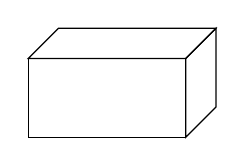
\begin{tikzpicture}
        \pgfmathsetmacro{\cubex}{2}
        \pgfmathsetmacro{\cubey}{1}
        \pgfmathsetmacro{\cubez}{1}
        \draw (0,0,0) -- ++(-\cubex,0,0) -- ++(0,-\cubey,0) -- ++(\cubex,0,0) -- cycle;
        \draw (0,0,0) -- ++(0,0,-\cubez) -- ++(0,-\cubey,0) -- ++(0,0,\cubez) -- cycle;
        \draw (0,0,0) -- ++(-\cubex,0,0) -- ++(0,0,-\cubez) -- ++(\cubex,0,0) -- cycle;
    \end{tikzpicture}
\end{theorem}



\end{document}